% ============================================================
%  heatmap_exp2.tex
%
%  Stand-alone compilable figure: FIFO vs RVI routing heatmap
%  for Experiment 2 (asymmetric costs, 2 fully flexible servers).
%
%  Configuration
%    tick_rate = 3,  lambda = (0.25, 0.25),  mu = 0.35
%    c = (100, 300),  D_0 = 6,  D_1 = 3  (physical time units)
%    => D0_ticks = 18 (outside visible range),  D1_ticks = 9
%
%  Axis orientation:
%    X-axis: FIL_1  (left=0, right=12)
%    Y-axis: FIL_0  (bottom=0, top=12)   <- natural
%
%  RVI blue cells derived from the actual computed action map.
%  Decoding rule for the text heatmap printout:
%    "0" -> FIFO-top was type 0, action=assign  -> blue
%    "1" -> FIFO-top was type 1, action=assign  -> orange
%    "." above diagonal (FIL_1 > FIL_0)         -> skip type 1, serve type 0 -> blue
%    "." on/below diagonal (FIL_0 >= FIL_1)     -> skip type 0, serve type 1 -> orange
% ============================================================
\documentclass[11pt,a4paper]{article}
\usepackage{tikz}
\usepackage{amsmath}
\usepackage[margin=2cm]{geometry}
\begin{document}

\begin{figure}[htbp]
\centering
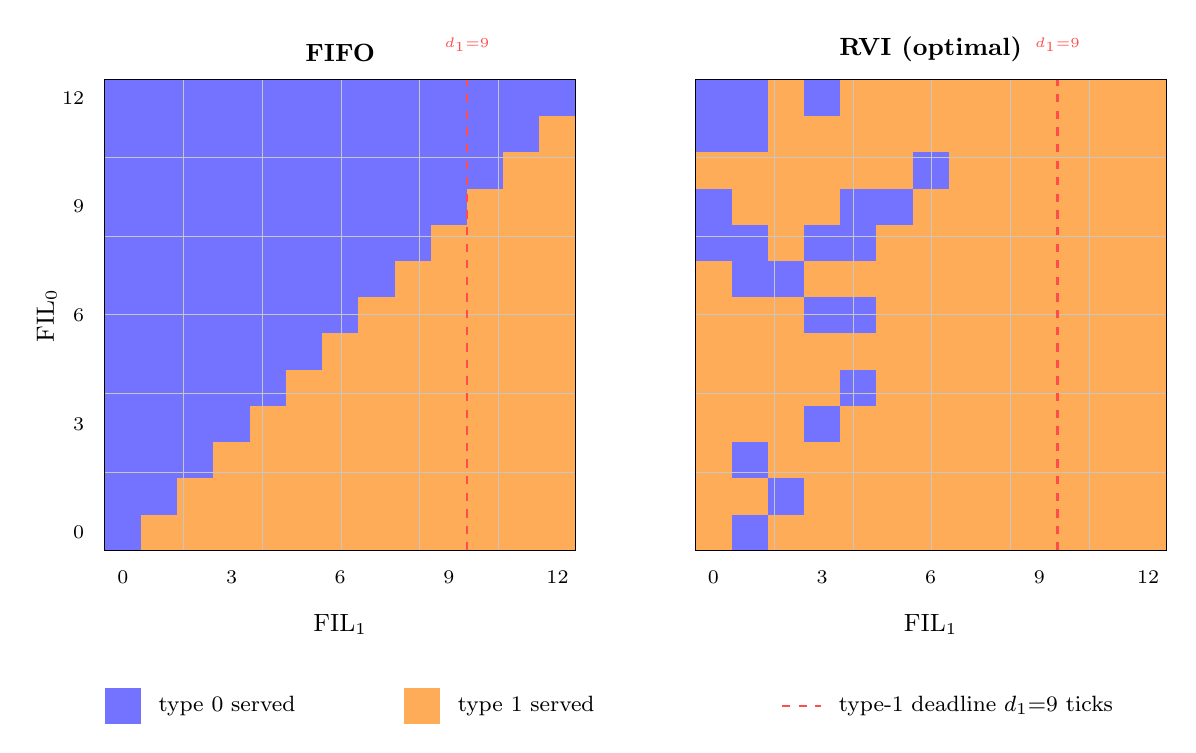
\begin{tikzpicture}[x=0.46cm, y=0.46cm]

  % ============================================================
  % LEFT PANEL — FIFO policy
  %
  % Always serves the oldest waiting job (highest FIL).
  %   FIL_0 >= FIL_1  =>  type 0 is FIFO-top  =>  blue
  %   FIL_1  > FIL_0  =>  type 1 is FIFO-top  =>  orange
  % ============================================================
  \begin{scope}

    \foreach \i in {0,...,12}{       % \i = FIL_0 (row, y-axis, 0 at bottom)
      \foreach \j in {0,...,12}{     % \j = FIL_1 (col, x-axis, 0 at left)
        \ifnum\i<\j
          \fill[orange!65] (\j,\i) rectangle (\j+1,\i+1);
        \else
          \fill[blue!55]   (\j,\i) rectangle (\j+1,\i+1);
        \fi
      }
    }

    \draw[gray!45, very thin] (0,0) grid (13,13);

    % Deadline: type-1 cost fires for FIL_1 > 9 (d_1 = 9 ticks)
    \draw[red!70, dashed, thick] (10,0) -- (10,13);
    \node[red!70, font=\tiny, above] at (10,13.5) {$d_1{=}9$};

    \foreach \j in {0,3,6,9,12}
      \node[below, font=\scriptsize] at (\j+0.5,-0.3) {\j};
    \foreach \i in {0,3,6,9,12}
      \node[left, font=\scriptsize] at (-0.3,\i+0.5) {\i};

    \node[below=5pt, font=\small] at (6.5,-1.1) {$\mathrm{FIL}_1$};
    \node[rotate=90, font=\small] at (-1.6,6.5) {$\mathrm{FIL}_0$};

    \draw[black, thin] (0,0) rectangle (13,13);
    \node[font=\small\bfseries, above=3pt] at (6.5,13) {FIFO};

  \end{scope}

  % ============================================================
  % RIGHT PANEL — RVI optimal policy
  %
  % Blue cells are taken directly from the computed action map.
  % Each entry below is (FIL_1=j / FIL_0=i), i.e. TikZ (x=j, y=i).
  %
  % Full decoded output (B=blue, O=orange):
  %   row  0: O B O O O O O O O O O O O  <- j=1 blue (. above diag)
  %   row  1: O O B O O O O O O O O O O  <- j=2 blue (. above diag)
  %   row  2: O B O O O O O O O O O O O  <- j=1 blue (0 below diag)
  %   row  3: O O O B O O O O O O O O O  <- j=3 blue (0 on diag)
  %   row  4: O O O O B O O O O O O O O  <- j=4 blue (0 on diag)
  %   row  5: O O O O O O O O O O O O O  <- all orange
  %   row  6: O O O B B O O O O O O O O  <- j=3,4 blue (0 below diag)
  %   row  7: O B B O O O O O O O O O O  <- j=1,2 blue (0 below diag)
  %   row  8: B B O B B O O O O O O O O  <- j=0,1,3,4 blue
  %   row  9: B O O O B B O O O O O O O  <- j=0,4,5 blue
  %   row 10: O O O O O O B O O O O O O  <- j=6 blue
  %   row 11: B B O O O O O O O O O O O  <- j=0,1 blue
  %   row 12: B B O B O O O O O O O O O  <- j=0,1,3 blue
  % ============================================================
  \begin{scope}[xshift=7.5cm]

    % Background: type 1 served everywhere
    \fill[orange!65] (0,0) rectangle (13,13);

    % Blue cells: exact RVI action map (format: FIL_1/FIL_0 = j/i)
    \foreach \j/\i in {
      1/0,
      2/1,
      1/2,
      3/3,
      4/4,
      3/6, 4/6,
      1/7, 2/7,
      0/8, 1/8,      3/8, 4/8,
      0/9,           4/9, 5/9,
      6/10,
      0/11, 1/11,
      0/12, 1/12,    3/12
    }{
      \fill[blue!55] (\j,\i) rectangle (\j+1,\i+1);
    }

    \draw[gray!45, very thin] (0,0) grid (13,13);

    \draw[red!70, dashed, thick] (10,0) -- (10,13);
    \node[red!70, font=\tiny, above] at (10,13.5) {$d_1{=}9$};

    \foreach \j in {0,3,6,9,12}
      \node[below, font=\scriptsize] at (\j+0.5,-0.3) {\j};
    \node[below=5pt, font=\small] at (6.5,-1.1) {$\mathrm{FIL}_1$};

    \draw[black, thin] (0,0) rectangle (13,13);
    \node[font=\small\bfseries, above=3pt] at (6.5,13) {RVI (optimal)};

  \end{scope}

  % ============================================================
  % Legend
  % ============================================================
  \begin{scope}[yshift=-2.2cm]
    \fill[blue!55]   (0cm,0cm) rectangle (0.46cm,0.46cm);
    \node[right, font=\footnotesize] at (0.56cm,0.23cm) {type~0 served};

    \fill[orange!65] (3.8cm,0cm) rectangle (4.26cm,0.46cm);
    \node[right, font=\footnotesize] at (4.36cm,0.23cm) {type~1 served};

    \draw[red!70, dashed, thick] (8.6cm,0.23cm) -- (9.1cm,0.23cm);
    \node[right, font=\footnotesize] at (9.2cm,0.23cm)
          {type-1 deadline $d_1{=}9$ ticks};
  \end{scope}

\end{tikzpicture}
\caption{%
  Routing decision heatmaps for Experiment~2
  ($\text{tick\_rate}=3$,\;
   $\boldsymbol{\lambda}=(0.25,0.25)$,\;
   $\mathbf{c}=(100,300)$,\;
   $D_0=6$, $D_1=3$ physical time units).
  Each cell $(i,j)$ shows which job type the server assigns when
  $\mathrm{FIL}_0=i$ (vertical axis, $0$ at bottom) and
  $\mathrm{FIL}_1=j$ (horizontal axis, $0$ at left).
  \textbf{Blue}: type~0 served.\quad\textbf{Orange}: type~1 served.
  \textbf{FIFO} (left) always serves the oldest job:
  blue on/above the diagonal ($\mathrm{FIL}_0 \ge \mathrm{FIL}_1$),
  orange below it.
  \textbf{RVI} (right) is dominated by type~1 (orange) throughout---reflecting
  its $3\times$ higher cost rate---but type~0 (blue) appears in scattered cells
  where the value function judges that type~0's age or proximity to its deadline
  tips the balance.
  Notably, a handful of blue cells sit \emph{above} the diagonal
  ($\mathrm{FIL}_1>\mathrm{FIL}_0$): RVI overrides FIFO order and serves the
  cheaper type because type~1's low FIL means it carries no urgency yet.
  The dashed red line marks $d_1=9$ ticks; type-1 cost accrues
  to the right of this line.%
}
\label{fig:heatmap_exp2}
\end{figure}

\end{document}
